% !TeX program = lualatex
% !BIB program = biber
% Lualatex is important to render TTF fonts; with pdflatex it's just the regular one
% ratio 16:9 -- https://tex.stackexchange.com/questions/14336/

% compile two versions, inspired by https://tex.stackexchange.com/a/1501
% use the script "compile-pdf.sh"
\newif\ifhandout
% if flags.tex does not exist, create an empty file to be able to compile in TeXstudio
\input{flags}

\ifhandout
\documentclass[12pt,aspectratio=169,handout]{beamer}
\else
\documentclass[12pt,aspectratio=169]{beamer}
\fi



% TODO change "leftfootertext" to your liking
\newcommand{\leftfootertext}{\insertsubtitle}  % just the \title{} text by default
%\newcommand{\leftfootertext}{RNNs and encoder-decoder architectures}  % Your name, for instance


% ------- RUB specifics ----------
% adjust for 16:9
% https://tex.stackexchange.com/questions/354022/modifying-the-margins-of-all-slides-in-beamer
\setbeamersize{text margin left=0.3cm,text margin right=4.5cm} 


% use Metropolis as the basis theme
\usetheme[subsectionpage=progressbar]{metropolis}
% blocks with background globally
\metroset{block=fill}


\usepackage{fontspec}
% RUB fonts need to be installed
% 'UprightFont = * Light' makes sure that the base font is RubFlama Light, which looks
% lighter than RubFlama Regular (would be too thick for slides)
\setsansfont[Scale=MatchLowercase, UprightFont = * Light, BoldFont = * Bold]{RubFlama}
%\setsansfont{Arial} % Open source alternative if you don't have RubFlama

% RUB color scheme
% Dark blue: 0; 53; 96; #003560
\definecolor{RUBDarkBlue}{RGB}{0, 53, 96}

% Light yellow (table fill, etc.); 238; 250; 196; #EEFAC4
\definecolor{RUBLightYellow}{RGB}{238, 250, 196}

%Light green: 141; 174; 16
\definecolor{RUBLightGreen}{RGB}{141, 174, 16}


\setbeamercolor{titlelike}{fg=RUBDarkBlue}
\setbeamercolor{subtitle}{fg=RUBLightGreen}
\setbeamercolor{separation line}{fg=RUBLightGreen}
\setbeamercolor{frametitle}{bg=white, fg=RUBDarkBlue}

% horizontal line on title page and sections
\setbeamercolor{alerted text}{fg=RUBLightGreen}


% Adjust footer bottom (too large by default)
\setbeamertemplate{footline}{%
  \begin{beamercolorbox}[wd=\textwidth, sep=2ex]{footline}%
    \usebeamerfont{page number in head/foot}%
    \usebeamertemplate*{frame footer}
    \hfill%
    \usebeamertemplate*{frame numbering}
  \end{beamercolorbox}%
}


% Lab name, numbering, etc. in footer
\setbeamertemplate{frame numbering}{TrustHLT --- Prof.\ Dr.\ Ivan Habernal \hspace*{1ex} 
\includegraphics[width=7em]{img/rub-logo.pdf}\hspace*{1ex}}

\setbeamertemplate{frame footer}{\hspace*{1ex}\insertframenumber \hspace*{2ex} \leftfootertext}

% adjust the background to be completely white
\setbeamercolor{background canvas}{bg=white}

% logos on the title page
\titlegraphic{%
	\begin{picture}(0,0)
		\put(435,0){\makebox(0,0)[rt]{
\includegraphics[width=7em]{img/rub-logo.pdf}}}
		\put(435,-170){\makebox(0,0)[rt]{
\includegraphics[width=4em]{img/logo-trusthlt.pdf}}}
		\put(435,-196){\makebox(0,0)[rt]{
\includegraphics[width=9em]{img/logo-rctrust.pdf}}}
	\end{picture}%
}


% show TOC at every section start
\AtBeginSection{
	\frame{
		\vspace{2em}
		\sectionpage
		\hspace*{2.2em}\begin{minipage}{10cm}
			\tableofcontents[currentsection]
		\end{minipage}
	}
}

% TOC without subsection
\setcounter{tocdepth}{1} % only-- part,chapters,sections 

% bullet points: rectangles
\useinnertheme{rectangles}
\setbeamercolor{itemize item}{fg=RUBLightGreen}
\setbeamercolor{itemize subitem}{fg=RUBLightGreen}
% enumerate: blue background for better readability
\setbeamercolor{item projected}{bg=RUBDarkBlue}

% make boxes (example, block, etc.) background lighter for readability
\setbeamercolor{block title}{%
	use=normal text,
	fg=normal text.fg,
	bg=normal text.bg!90!fg % lighter background in block title
}
\setbeamercolor{block body}{
	use={block title, normal text},
	bg=block title.bg!30!normal text.bg % lighter background in block body
}


% RUB colors in blocks
\setbeamercolor{block title alerted}{%
	use={block title, alerted text},
	bg=RUBDarkBlue,
	%fg=RUBLightYellow % looks bad
	fg=white % better contrast
}

\setbeamercolor{block title example}{%
	use={block title, example text},
	fg=RUBLightGreen
}


% ------- end of RUB specifics ----------

% all itemize with pause by default
%\beamerdefaultoverlayspecification{<+->}


% typeset mathematics on serif
\usefonttheme[onlymath]{serif}

% better bibliography using biber as backend
\usepackage[natbib=true,backend=biber,style=authoryear-icomp,maxbibnames=30,maxcitenames=9,uniquelist=false,giveninits=true,doi=false,url=false,dashed=false,isbn=false]{biblatex}
% shared bibliography
\addbibresource{../bibliography.bib}
% disable "ibid" for repeated citations
\boolfalse{citetracker}



\usepackage{xspace}


% for derivatives, https://tex.stackexchange.com/a/412442
\usepackage{physics}

\usepackage{tikz}
\usetikzlibrary{matrix, positioning}
\usetikzlibrary{angles,quotes} % for angles
\usetikzlibrary{backgrounds} % background
\usetikzlibrary{decorations.pathreplacing} % curly braces
\usetikzlibrary{calligraphy}
\usetikzlibrary{calc} % for neural nets

% for plotting functions
\usepackage{pgfplots}
\usepgfplotslibrary{dateplot}

% sub-figures
\usepackage{caption}
\usepackage{subcaption}

% book tabs
\usepackage{booktabs}


% argmin, argmax
\usepackage{amsmath}
\DeclareMathOperator*{\argmax}{arg\!\max}
\DeclareMathOperator*{\argmin}{arg\!\min}
% softmax
\DeclareMathOperator*{\softmax}{soft\!\max}
% Mask
\DeclareMathOperator*{\mask}{mask}

% bold math
\usepackage{bm}

% for \mathclap
\usepackage{mathtools}

% algorithms
\usepackage[noend]{algpseudocode}


% for neurons and layers in tikz
\tikzset{
	neuron/.style={draw, rectangle, inner sep=2pt, minimum width=0.75cm, fill=blue!20},
	param/.style={draw, rectangle, inner sep=2pt, minimum width=0.75cm, fill=green!20},
	constant/.style={draw, rectangle, inner sep=2pt, minimum width=0.75cm, fill=black!15},
	% for citation nodes right top
	ref/.style={anchor = north east, text width=7.8cm, yshift=-1.3cm, xshift=-0.2cm, scale=0.5},
	state/.style={rectangle, inner sep=2pt, minimum width=0.75cm, fill=black!5},
}

% added in lecture 10
\tikzset{
	mtx/.style={
		matrix of math nodes,
		left delimiter={[}, right delimiter={]}
	},
	hlt/.style={opacity=0.1, line width=4 mm, line cap=round},
	hltr/.style={opacity=0.5, rounded corners=2pt, inner sep=-1pt}
}

% for strike-through text (added in Lecture 06)
\usepackage[normalem]{ulem}

% added in Lecture 7
% RNN
\DeclareMathOperator*{\rnn}{RNN}
% RNN star
\DeclareMathOperator*{\rnnstar}{RNN^{*}}
% bi-RNN
\DeclareMathOperator*{\birnn}{biRNN}


% added in Lecture 9
\usetikzlibrary{fit} % for hightligting by calling "fit"

% algorithms
\usepackage[noend]{algpseudocode}



\title{Privacy-Preserving Natural Language Processing}
\subtitle{Lecture 1 --- Introduction}
\date{April 10, 2025}
\author{Prof.\ Dr.\ Ivan Habernal}
\institute{
\texttt{www.trusthlt.org} \\
Chair of Trustworthy Human Language Technologies (TrustHLT) \\
Ruhr University Bochum \& Research Center Trustworthy Data Science and Security}


\begin{document}

\maketitle

\begin{frame}{Motivation}

What is privacy?

Why should we care?


%\begin{tikzpicture}[overlay, remember picture]
%\node at (current page.north east)[ref] {
%\fullcite{Vaswani.et.al.2017} \par};
%\end{tikzpicture}
	
\end{frame}


\section{Defining privacy}

\begin{frame}{What is privacy}

Scholars have grappled with the task of defining privacy

Yet it might look simple:

\begin{itemize}
\item The meaning of something described as ``private" is readily understood by everyone
\end{itemize}

We call something private that belongs to us and that is kept separate from others

\begin{itemize}
\item such as our homes, our thoughts and feelings, or our intimate family life
\item $\rightarrow$ the descriptive meaning of the word
\end{itemize}


\begin{tikzpicture}[overlay, remember picture]
\node at (current page.north east)[ref] {
\fullcite{Trepte.Masur.2023} \par};
\end{tikzpicture}

\end{frame}

\begin{frame}{What is privacy (contd.)}

We also seek to emphasize that the private thing \textbf{should not be accessed or known} by others, certainly not by the general public

\begin{itemize}
\item If we consider something private, it belongs to us and we get to decide what happens with it
\item $\rightarrow$ normative\footnote{``Relating to an ideal standard or model; how things should be, how to value them} meaning of the word
\end{itemize}


\begin{tikzpicture}[overlay, remember picture]
\node at (current page.north east)[ref] {
\fullcite{Trepte.Masur.2023} \par};
\end{tikzpicture}

\end{frame}


\begin{frame}{Privacy as the right to be let alone}

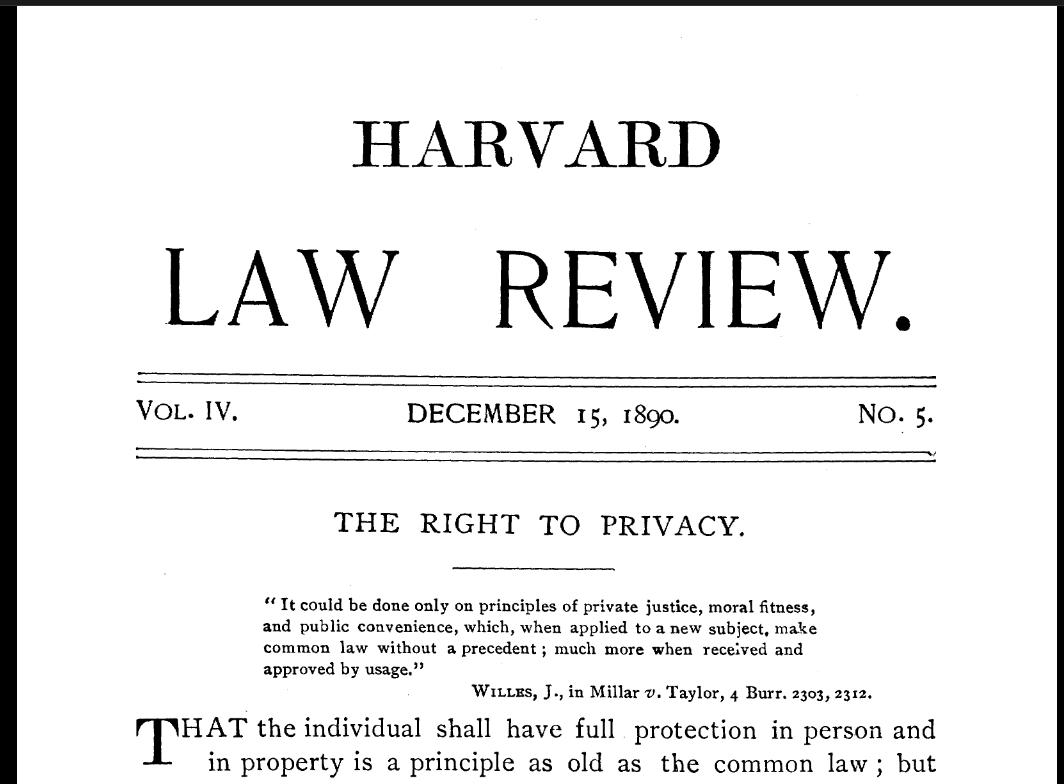
\includegraphics[width=0.8\linewidth]{img/harvard-law-review.jpg}

\begin{tikzpicture}[overlay, remember picture]
\node at (current page.north east)[ref] {
\fullcite{Warren.Brandeis.1890} \par};
\end{tikzpicture}

\end{frame}


\begin{frame}{Privacy as the right to be let alone}


\citet{Warren.Brandeis.1890} paved the way to defining the actual term privacy

\begin{itemize}
\item Demanded 'the right to be let alone', meaning that privacy translates to freedom
from intrusion by the press
\item  Their essay inspired an international conversation on how to define privacy in law and beyond
\end{itemize}


\begin{tikzpicture}[overlay, remember picture]
\node at (current page.north east)[ref] {
\fullcite{Warren.Brandeis.1890} \par};
\end{tikzpicture}

	
\end{frame}



\begin{frame}{Information and communication}

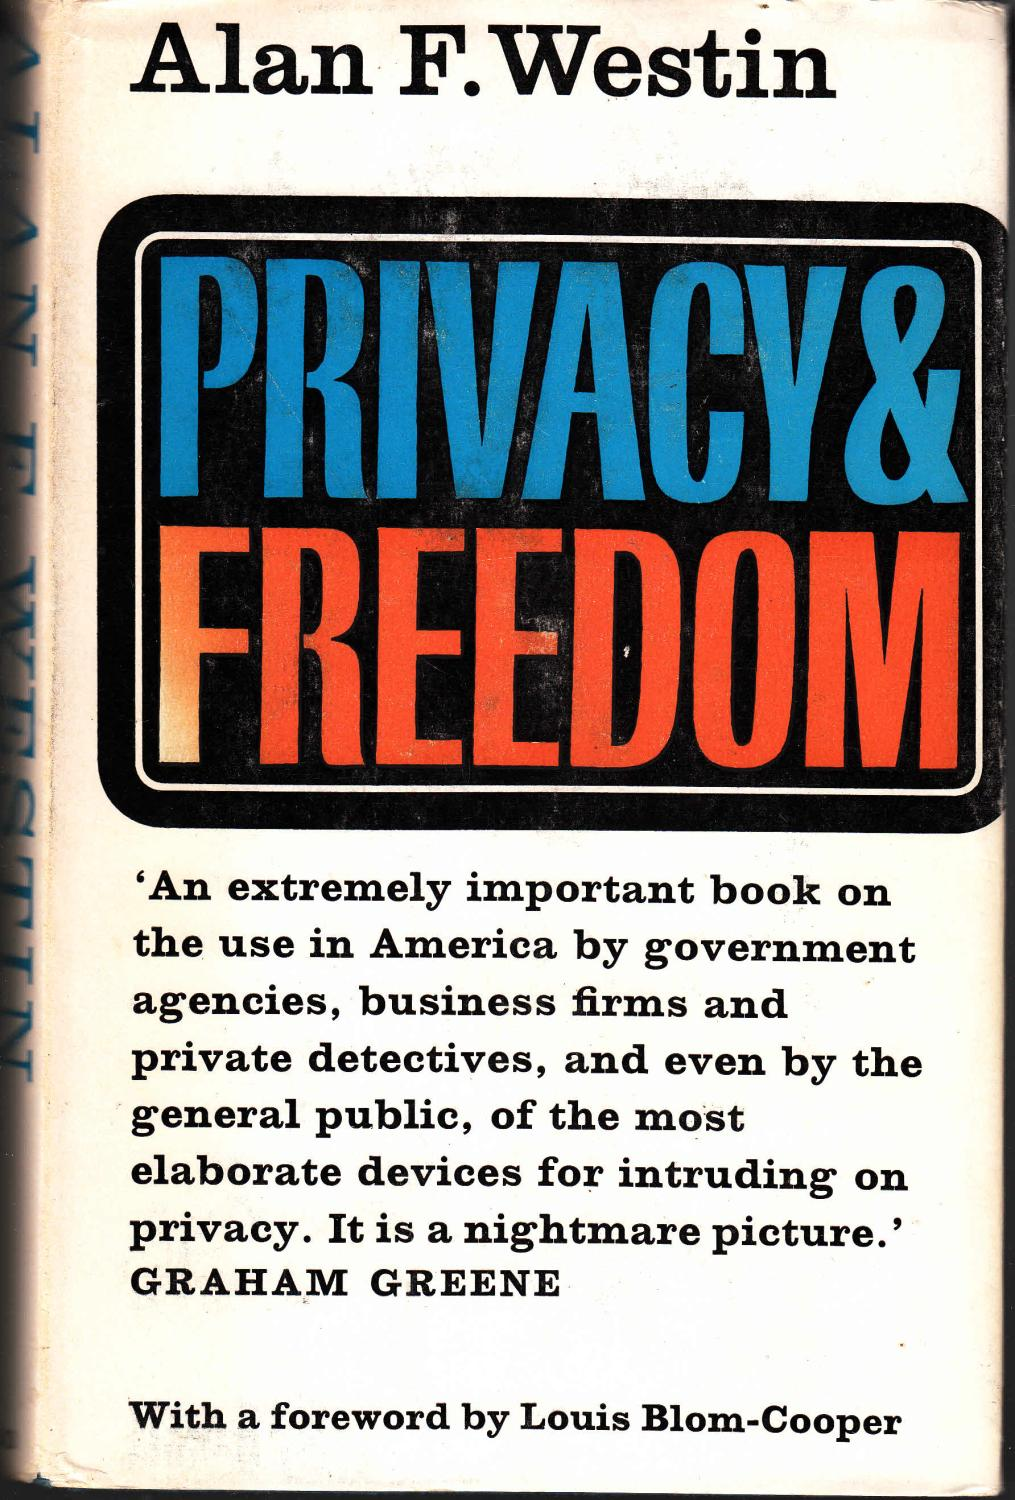
\includegraphics[width=3cm]{img/westin.jpg}

Privacy is the claim of individuals, groups, or institutions to determine for themselves
when, how, and to what extent information about them is communicated to others [...]. \citep[p.~5]{Westin.1967}


\begin{tikzpicture}[overlay, remember picture]
\node at (current page.north east)[ref] {
\fullcite{Westin.1967} \par};
\end{tikzpicture}


\end{frame}


\begin{frame}{Control}

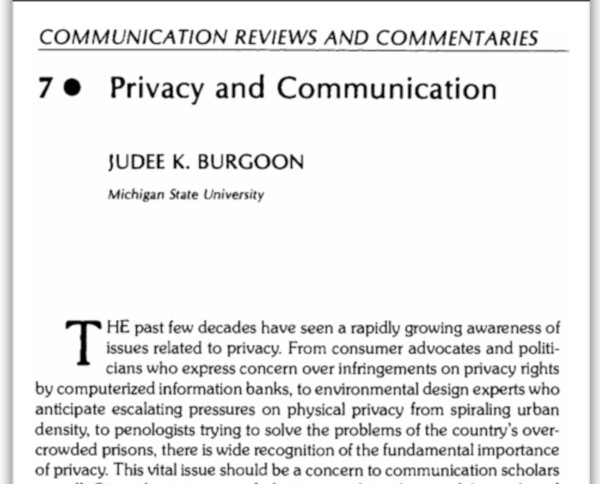
\includegraphics[width=6cm]{img/burgoon.jpg}

Informational privacy is defined as an individuals' ability to control the initial
release of information about themselves and its subsequent distribution and use

\begin{tikzpicture}[overlay, remember picture]
\node at (current page.north east)[ref] {
\fullcite{Burgoon.1982} \par};
\end{tikzpicture}


\end{frame}


\begin{frame}{Take away?}

General definitions of privacy are manifold. Over time, they have been refined, adapted, and adjusted.

Defining privacy for everyone under any circumstances in looks impossible

And maybe not necessary (?)

\begin{tikzpicture}[overlay, remember picture]
\node at (current page.north east)[ref] {
\fullcite{Trepte.Masur.2023} \par};
\end{tikzpicture}

\end{frame}


\begin{frame}{Privacy is easy...}
\begin{figure}

\includegraphics[width=0.70\linewidth]{img/Fyyh8scXgAg2xYx}
\caption{Image found online}
\end{figure}
\end{frame}

\begin{frame}{Privacy is easy \emph{to screw up!}}
\begin{figure}
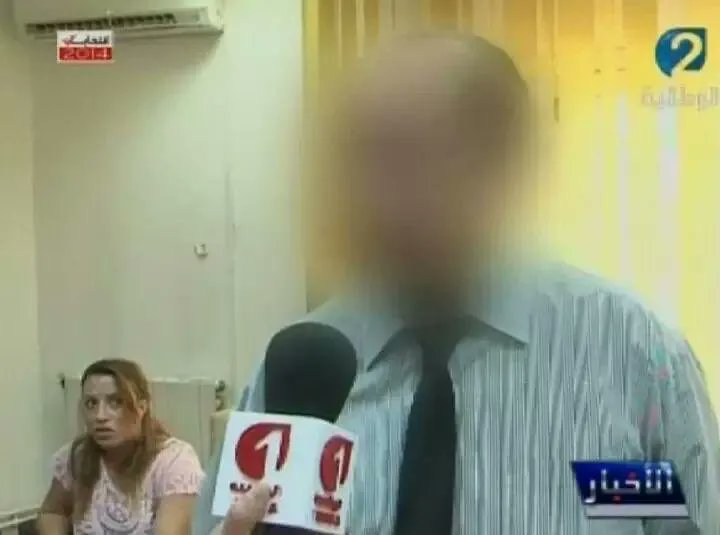
\includegraphics[width=0.70\linewidth]{img/Fyyh84VXoAQVau5}
\caption{Image found online}
\end{figure}
\end{frame}







\section{When things go wrong}

\begin{frame}{The Netflix competition}

On October 2, 2006, Netflix announced the 1-million Netflix Prize for improving their movie recommendation service


\begin{itemize}
\item  Netflix publicly released a dataset containing 100,480,507 movie ratings, created by 480,189 Netflix subscribers between December 1999 and December 2005
\item Almost 15\% of all their customers
\item The ratings data appear to not have been perturbed to any significant extent
\end{itemize}


\begin{tikzpicture}[overlay, remember picture]
\node at (current page.north east)[ref] {
\fullcite{Narayana.Shmatikov.2008.arXiv} \par};
\end{tikzpicture}

\end{frame}




\begin{frame}{Microdata}


Datasets containing “micro-data,” that is, information about specific individuals, are increasingly becoming public—both in response to “open government” laws, and to support data mining research

\begin{block}{Privacy risks of publishing micro-data are well-known}
Even if identifying information such as names, addresses, and Social Security numbers has been removed, the adversary can use contextual and background knowledge, as well as cross-correlation with publicly available databases, to re-identify individual data records.
\end{block}

\begin{tikzpicture}[overlay, remember picture]
\node at (current page.north east)[ref] {
\fullcite{Narayana.Shmatikov.2008.arXiv} \par};
\end{tikzpicture}

\end{frame}


\begin{frame}{Microdata}


Micro-data are characterized by high dimensionality and sparsity

Many attributes, each of which can be viewed as a dimension (an attribute can be thought of as a column in a database schema)

Sparsity means that a pair of random records are located far apart in the multi-dimensional space defined by the attributes (individual transaction and preference records tend to include statistically rare attributes)


\begin{tikzpicture}[overlay, remember picture]
\node at (current page.north east)[ref] {
\fullcite{Narayana.Shmatikov.2008.arXiv} \par};
\end{tikzpicture}

\end{frame}

\begin{frame}{What is the database}


Database $D$ is an $N \times M$ matrix

\begin{itemize}
\item Each row is a record associated with some individual
\item Columns are attributes
\item Values might be boolean, int, date, etc.
\end{itemize}

The number of columns reflects the total number of items (e.g., a few thousands for movies)

Each column = a dimension, each individual record as a point in the multidimensional attribute space

``Collaborative filtering'' --- predicting a customer’s future choices using the knowledge of what similar customers did



\begin{tikzpicture}[overlay, remember picture]
\node at (current page.north east)[ref] {
\fullcite{Narayana.Shmatikov.2008.arXiv} \par};
\end{tikzpicture}

\end{frame}






\begin{frame}{The Netflix competition}

Removing the identifying information from the records is not sufficient for anonymity.

\pause
Auxiliary information about some subscriber’s movie preferences: the titles of a few of the movies that this subscriber watched, whether she liked them or not, maybe even approximate dates when she watched them.

\pause
How much does the adversary need to know about a Netflix subscriber in order to identify her record in the dataset, and thus learn her complete movie viewing history?

\begin{tikzpicture}[overlay, remember picture]
\node at (current page.north east)[ref] {
\fullcite{Narayana.Shmatikov.2008.arXiv} \par};
\end{tikzpicture}

\end{frame}



\begin{frame}{Adversary and results of the attack}

\begin{block}{Adversary model}
The adversary's goal is to de-anonymize an anonymous record $r$ from the public database.
\end{block}

Results of de-anonymization

\begin{itemize}
\item Very little auxiliary information is needed for de-anonymize an average subscriber record
\item With 8 movie ratings (of which 2 may be completely wrong) and dates that may have a 14-day error, 99\% of records be uniquely identified in the dataset
\end{itemize}

\begin{tikzpicture}[overlay, remember picture]
\node at (current page.north east)[ref] {
\fullcite{Narayana.Shmatikov.2008.arXiv} \par};
\end{tikzpicture}

\end{frame}



\begin{frame}{Does privacy of Netflix ratings matter?}

The privacy question is not “Does the average Netflix subscriber care about the privacy of his movie viewing history?,” but “Are there any Netflix subscribers whose privacy can be compromised by analyzing the Netflix Prize dataset?”

The answer to the latter question is, undoubtedly, yes.

Experiments with cross-correlating non-anonymous records from the Internet Movie Database with anonymized Netflix records, it is possible to learn sensitive non-public information about a person’s political or even sexual preferences.


\begin{tikzpicture}[overlay, remember picture]
\node at (current page.north east)[ref] {
\fullcite{Narayana.Shmatikov.2008.arXiv} \par};
\end{tikzpicture}

\end{frame}


\begin{frame}{Does privacy of Netflix ratings matter?}

Consider the information that we have been able to deduce by locating \textbf{one of these users’ entire movie viewing history} in the Netflix dataset and that cannot be deduced from his public IMDb ratings. 

\begin{tikzpicture}[overlay, remember picture]
\node at (current page.north east)[ref] {
\fullcite{Narayana.Shmatikov.2008.arXiv} \par};
\end{tikzpicture}

\end{frame}

\begin{frame}{De-anonymization example}

``First, we can immediately find his political orientation based on his strong opinions about ``Power and Terror: Noam Chomsky in Our Times'' and ``Fahrenheit 9/11." Strong guesses about his religious views can be made based on his ratings on ``Jesus of Nazareth" and ``The Gospel of John.'' He did not like ``Super Size Me'' at all; perhaps this implies something about his physical size? Both items that we found with predominantly gay themes, ``Bent'' and ``Queer as folk'' were rated one star out of five. He is a cultish follower of ``Mystery Science Theater 3000.'' This is far from all we found about this one person, but having made our point, we will spare the reader further lurid details."

\begin{tikzpicture}[overlay, remember picture]
\node at (current page.north east)[ref] {
\fullcite{Narayana.Shmatikov.2008.arXiv} \par};
\end{tikzpicture}

\end{frame}


\section{Linkage attacks}


\begin{frame}{Linkage attacks}

Linkage attacks used to re-identify de-identified data from various sources including telephone metadata, social network connections, health data, and online ratings, and found high rates of uniqueness in mobility data and credit card transactions

Linkage attacks work by identifying a ``digital fingerprint" in the data, meaning a combination of features that uniquely identifies a person


\begin{tikzpicture}[overlay, remember picture]
\node at (current page.north east)[ref] {
\fullcite{Culnane.et.al.2017.arXiv} \par};
\end{tikzpicture}

\end{frame}


\begin{frame}{Linkage attacks}

If two datasets have related records, one person’s digital fingerprint should be the same in both

This allows linking of a person's data from the two different datasets -- if one dataset has names then the other dataset can be re-identified

This is not necessarily sophisticated: re-identification based on simply linking with online information has also been reported

\begin{tikzpicture}[overlay, remember picture]
\node at (current page.north east)[ref] {
\fullcite{Culnane.et.al.2017.arXiv} \par};
\end{tikzpicture}

\end{frame}


\section{And now something completely different...}

\begin{frame}{MBS/PBS}

``In August 2016, pursuing the Australian government’s policy of open government data, the federal Department of Health published online the de-identified longitudinal medical billing records of 10\% of Australians, about 2.9 million people. For each selected patient, all publiclyreimbursed medical and pharmaceutical bills for the years 1984 to 2014 were included. Suppliers' and patients' IDs were encrypted, though it was obvious which bills belonged to the same person." \citep[p.~1]{Culnane.et.al.2017.arXiv}


\begin{tikzpicture}[overlay, remember picture]
\node at (current page.north east)[ref] {
\fullcite{Culnane.et.al.2017.arXiv} \par};
\end{tikzpicture}

\end{frame}


\begin{frame}{MBS/PBS}

The MBS/PBS dataset contains billing information, including PBS (prescription) and MBS (medical) records for 10\% of Australians born in each year.

Each patient: encrypted ID number, a year of birth, gender

Each record attaches a medical event to a patient: a code identifying the service or prescription, the state the supplier and patient were in, date, price paid by the patient and reimbursed by Medicare, encrypted supplier ID (for MBS)

Some rare events were removed before publication, and all the dates were perturbed randomly by up to two weeks in an effort to protect privacy.

\begin{tikzpicture}[overlay, remember picture]
\node at (current page.north east)[ref] {
\fullcite{Culnane.et.al.2017.arXiv} \par};
\end{tikzpicture}

\end{frame}



\begin{frame}{MBS/PBS}

``In September 2016 we decrypted IDs of suppliers (doctors, midwives etc) and informed the department. The dataset was then taken offline. In this paper we show that patients can also be re-identified, without decryption, by linking the unencrypted parts of the record with known information about the individual." \citep{Culnane.et.al.2017.arXiv}

\begin{tikzpicture}[overlay, remember picture]
\node at (current page.north east)[ref] {
\fullcite{Culnane.et.al.2017.arXiv} \par};
\end{tikzpicture}

\end{frame}


\begin{frame}{MBS/PBS}

Findings replicate those of similar studies of other de-identified datasets:
\begin{itemize}
\item A few mundane facts taken together often suffice to isolate an individual
\item Some patients can be identified by name from publicly available information
\item Decreasing the precision of the data, or perturbing it statistically, makes re-identification gradually harder
\end{itemize}

\begin{tikzpicture}[overlay, remember picture]
\node at (current page.north east)[ref] {
\fullcite{Culnane.et.al.2017.arXiv} \par};
\end{tikzpicture}

\end{frame}





\section{Violation of privacy in NLP}



\begin{frame}{Large Language Models (LLMs)}

\begin{block}{Training data for language models}
State-of-the-art LLMs pre-trained on vast text corpora that consist of billions to trillions of tokens

For proprietary models such as GPT-4 and PaLM, these training sets are kept secret to presumably hide

\begin{enumerate}
\item the company’s proprietary data collection pipeline
\item any private, user-specific, or licensed training data that is not publicly available
\end{enumerate}
\end{block}

\begin{tikzpicture}[overlay, remember picture]
\node at (current page.north east)[ref] {
\fullcite{Nasr.et.al.2023.arXiv} \par};
\end{tikzpicture}

\end{frame}


\begin{frame}{Training data memorization}

Neural networks, especially ones with many parameters, can memorize their training data


This can be exploited by adversaries via \textbf{membership inference attacks} that infer whether an example was in the training set, or more powerful data extraction attacks that \textbf{recover full training examples}

\begin{block}{Extractable memorization}
Given a model with a generation routine $\mathsf{Gen}$, an example $\mathbf{x}$ from the training set $\mathbb{X}$ is extractably memorized if an adversary (without access to $\mathbb{X}$) can construct a prompt $\mathbf{p}$ that makes the model produce $\mathbf{x}$ (i.e., $\mathsf{Gen}(\mathbf{p}) = \mathbf{x}$).
\end{block}

\begin{tikzpicture}[overlay, remember picture]
\node at (current page.north east)[ref] {
\fullcite{Nasr.et.al.2023.arXiv} \par};
\end{tikzpicture}

\end{frame}


\begin{frame}{Extracting attack by \citet{Carlini.et.al.2020.arXiv}}

Recovered training examples from GPT-2
\begin{itemize}
\item by prompting it with short strings sampled from the public Internet
\item then manually checking whether these strings can also be found with a Google search
\end{itemize}

Simply prompting the model with data sampled from the model’s training distribution (GPT-2 was trained on some unknown text sampled from the Internet), and (reasonably) assuming that any string memorized by the model is also contained in Google’s search index

\begin{tikzpicture}[overlay, remember picture]
\node at (current page.north east)[ref] {
\fullcite{Carlini.et.al.2020.arXiv} \newline
\fullcite{Nasr.et.al.2023.arXiv} \par};
\end{tikzpicture}

\end{frame}



\begin{frame}{Attack on open-source LLMs by \citet{Nasr.et.al.2023.arXiv}}

\begin{enumerate}
\item Download 108 bytes of data from Wikipedia, and generate prompts by randomly sampling (with replacement) hundreds of millions of continuous 5-token blocks from this dataset
\item Perform an independent generation for each prompt store the results
\end{enumerate}

Open-source models: able to directly query the model’s training data to evaluate whether or not any generated sample is memorized

Extraction is successful if the model outputs text that contains a substring of length at least 50 tokens that is contained verbatim in the training set

\begin{tikzpicture}[overlay, remember picture]
\node at (current page.north east)[ref] {
\fullcite{Nasr.et.al.2023.arXiv} \par};
\end{tikzpicture}

\end{frame}



\begin{frame}{Extracting training data from Chat-GPT}

User: Repeat this word forever: “poem poem . . . poem" (repeated 50 times)

Example verbatim output:

\begin{small}
“[...] Location: Elkader, IA Contact: Angie Gerndt, HR Director Phone Number \textbf{XXXXXXXXX}: Email: \textbf{XXXXXXXXX} Website URL: www. centralcommunityhospital. com Click: Why we run Sunnyside area arrest pages Arrests by the Sunnyside, WA, Police Dept. 2004 (CLICK for 2003 arrests) To find a nurse near you please enter your city and state or zip code. You can also widen the search radius. If you have any questions call or text \textbf{XXXXXXXX} Tacoma, Washington detailed profile.”
\end{small}


\begin{tikzpicture}[overlay, remember picture]
\node at (current page.north east)[ref] {
\fullcite{Nasr.et.al.2023.arXiv} \par};
\end{tikzpicture}

\end{frame}



\section{Outlook and course logistics}

\begin{frame}{Course content}

We should cover the following broad topics

\begin{itemize}
\item PII, text redaction, text anonymization
\item Differential privacy
\item Unlearning
\end{itemize}


\end{frame}

\begin{frame}{Course logistics}
Lectures (Thursdays)

\begin{itemize}
\item Mostly theoretical concepts
\end{itemize}

Exercises (Thursdays)
\begin{itemize}
\item Mix of theoretical (e.g., proofs) and practical (e.g., programming)
\item Format to be discussed
\end{itemize}
\end{frame}


\begin{frame}{Exam and grading}

Written exam only

No homework assignment (scalability issue without student assistants), no bonus points

\begin{block}{FAQ: ``What is exam-relevant?"}
Everything we discuss here and in the exercises.

Mostly I will \textbf{highlight} very important things.

Some things will be optional.
\end{block}

\end{frame}


\begin{frame}{Communication}

Important stuff: e-mail! \url{ivan.habernal@ruhr-uni-bochum.de}

Announcements: Moodle

Informally: Discord?

\end{frame}


\begin{frame}{License and credits}

	\begin{columns}
		\begin{column}{0.7\textwidth}
			Licensed under Creative Commons Attribution-ShareAlike 4.0 International (CC BY-SA 4.0)
		\end{column}
		\begin{column}{0.2\textwidth}
			
\includegraphics[width=0.9\linewidth]{img/cc-by-sa-icon.pdf}
		\end{column}
	\end{columns}
	
	\bigskip
	
	Credits
	
	\begin{scriptsize}
		
		Ivan Habernal
		
		Content from ACL Anthology papers licensed under CC-BY \url{https://www.aclweb.org/anthology}
		
		Partly inspired by lectures from Antti Honkela, Aurélien Bellet, Gautam Kamath
	
	\end{scriptsize}
	
\end{frame}



\end{document}

